\subsection{Opgave 54}

Figuren viser grafen for en funktion f. 

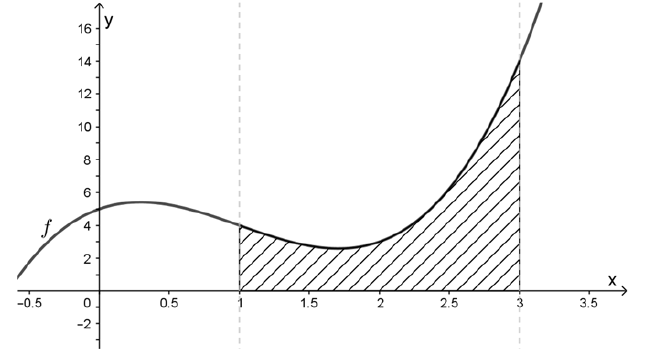
\includegraphics[width=8cm]{Opgave_51-56/Opgave_54/54.png}

Funktionen f er bestemt ved forskriften 

\begin{align*}
    f(x) = 2x^3 - 6x^2 +3x +5
\end{align*}

Det skraverede område på figuren angiver arealet af området afgrænset af x-aksen, f samt linjerne $x = 1$ og $x = 3$.

Bestem arealet af det skraverede område.

\ans

For at bestemme arealet af det skraverede område skal vi bestemme arealet under funktinen $f(x)$
fra x værdien $x = 1$ til x værdien $x = 3$.

For at bestemmet arealet under en kurve skal vi bruge formlen 

\begin{align*}
    \int_a^b f(x) dx = F(b) - F(a)
\end{align*}

Her er a værdien vores start x værdi og b værdien er vores slut x værdi.
$\int f(x) dx$ betyder integralet af funktionen $f(x)$ og $F(x)$ er resultatet vi får når vi integrerer $f(x)$. Der gælder følgende regler for integraler.

Hvis vi har en funktion på formen $f(x) = a\cdot x^n$ bliver ingetralet
$F(x) = \frac{a}{n + 1}x^{n + 1}$

Hvis vi har en konstant $f(x) = a$ bliver integralet 
$F(x) = a\cdot x$

Vi bestemmer nu arealet under kurven $f(x)$ hvor $a = 1$ og $b = 3$

\begin{align*}
    \int_1^3 2x^3 - 6x^2 +3x +5 dx &= \left[\frac{2}{3 + 1}x^{3+1} - \frac{6}{2 + 1}x^{2+1} + \frac{3}{1 + 1}x^{1+1} + 5x \right]_1^3 = \left[0,5x^4 - 2x^3 + 1,5x^2 + 5x\right]_1^3\\
    &= (0,5\cdot 3^4 - 2\cdot 3^3 + 1,5 \cdot 3^2 + 5\cdot 3) - (0,5 \cdot 1^4 - 2\cdot 1^3 + 1,5 \cdot 1^2 + 5 \cdot 1)\\
    &= 10
\end{align*}

Arealet af det skraverede område er derfor 10.